% questions.tex —— 2012 年·上海卷·理科 · 题目内容片段（无答案）
% 由 tools/generate_projects.py 依来源总账自 2012/2012_数学真题_上海理_试题.md 生成，勿手改（改源 MD 后重跑）

\gkpart{一、填空题}

\begin{question}
\gkti{1}计算：$\dfrac{3-\mathrm i}{1+\mathrm i}=$\gkblank{}。（$\mathrm i$ 为虚数单位）

\end{question}
\begin{question}
\gkti{2}若集合 $A=\{x\mid2x-1>0\}$，$B=\{x\mid|x-1|<2\}$，则 $A\cap B=$\gkblank{}。

\end{question}
\begin{question}
\gkti{3}函数 $f(x)=\begin{vmatrix}2&\cos x\\ \sin x&-1\end{vmatrix}$ 的值域是\gkblank{}。

\end{question}
\begin{question}
\gkti{4}若 $\overrightarrow n=(-2,1)$ 是直线 $l$ 的一个法向量，则 $l$ 的倾斜角的大小为\gkblank{}。（结果用反三角函数值表示）

\end{question}
\begin{question}
\gkti{5}在 $\left(x-\dfrac2x\right)^6$ 的二项展开式中，常数项等于\gkblank{}。

\end{question}
\begin{question}
\gkti{6}有一列正方体，棱长组成以 $1$ 为首项、$\dfrac12$ 为公比的等比数列，体积分别记为 $V_1$，$V_2$，$\cdots$，$V_n$，$\cdots$，则 $\lim\limits_{n\to\infty}(V_1+V_2+\cdots+V_n)=$\gkblank{}。

\end{question}
\begin{question}
\gkti{7}已知函数 $f(x)=\mathrm e^{|x-a|}$（$a$ 为常数）。若 $f(x)$ 在区间 $[1,+\infty)$ 上是增函数，则 $a$ 的取值范围是\gkblank{}。

\end{question}
\begin{question}
\gkti{8}若一个圆锥的侧面展开图是面积为 $2\pi$ 的半圆面，则该圆锥的体积为\gkblank{}。

\end{question}
\begin{question}
\gkti{9}已知 $y=f(x)+x^2$ 是奇函数，且 $f(1)=1$。若 $g(x)=f(x)+2$，则 $g(-1)=$\gkblank{}。

\Needspace{0.4\textheight}
\end{question}
\begin{question}
\gkti{10}如图，在极坐标系中，过点 $M(2,0)$ 的直线 $l$ 与极轴的夹角 $\alpha=\dfrac\pi6$。若将 $l$ 的极坐标方程写成 $\rho=f(\theta)$ 的形式，则 $f(\theta)=$\gkblank{}。
\nopagebreak[4]
\begin{center}% 2012 年上海卷理科第 10 题：极坐标系中过 M(2,0)、与极轴成 π/6 的直线 l。
% 来源 PDF：普通高考/2012/2012上海理.pdf，第 1 页（印面 767）第 1 栏。
% 重绘依据：原图为极坐标示意图：O 在左、极轴向右，M 在极轴上距 O 为 2，直线 l 过 M 且与极轴夹角 α。
\begin{tikzpicture}[scale=1.0, semithick, >=Stealth]
  \draw[->] (-0.6,0) -- (3.4,0) node[right] {$x$};
  \node[below left] at (0,0) {$O$};
  \fill (2,0) circle (1.5pt) node[below] {$M$};
  % 过 M、倾斜角 30° 的直线
  \draw (-0.35,-0.35*0.577) -- (3.1,1.1*0.577);
  \draw (2.55,0) arc[start angle=0, end angle=30, radius=0.55];
  \node at (2.95,0.22) {$\alpha$};
  \node[right] at (3.05,0.72) {$l$};
\end{tikzpicture}
\end{center}
\nopagebreak[4]
\end{question}
\begin{question}
\gkti{11}三位同学参加跳高、跳远、铅球项目的比赛。若每人都选择其中两个项目，则有且仅有两人选择的项目完全相同的概率是\gkblank{}。（结果用最简分数表示）

\end{question}
\begin{question}
\gkti{12}在平行四边形 $ABCD$ 中，$\angle A=\dfrac\pi3$，边 $AB$，$AD$ 的长分别为 $2$，$1$。若 $M$，$N$ 分别是边 $BC$，$CD$ 上的点，且满足 $\dfrac{|BM|}{|BC|}=\dfrac{|CN|}{|CD|}$，则 $\overrightarrow{AM}\cdot\overrightarrow{AN}$ 的取值范围是\gkblank{}。

\end{question}
\begin{question}
\gkti{13}已知函数 $y=f(x)$ 的图象是折线段 $ABC$，其中 $A(0,0)$，$B\left(\dfrac12,5\right)$，$C(1,0)$。函数 $y=xf(x)$（$0\leqslant x\leqslant1$）的图象与 $x$ 轴围成的图形的面积为\gkblank{}。

\Needspace{0.4\textheight}
\end{question}
\begin{question}
\gkti{14}如图，$AD$ 与 $BC$ 是四面体 $ABCD$ 中互相垂直的棱，$BC=2$。若 $AD=2c$，且 $AB+BD=AC+CD=2a$，其中 $a$，$c$ 为常数，则四面体 $ABCD$ 的体积的最大值是\gkblank{}。
\nopagebreak[4]
\begin{center}% 2012 年上海卷理科第 14 题：四面体 ABCD，AD 与 BC 为互相垂直的棱，BC=2。
% 来源 PDF：普通高考/2012/2012上海理.pdf，第 1 页（印面 767）第 2 栏。
% 重绘依据：原图为斜二测式透视：D 在上方偏左，A 在其左下方，C 在右侧，B 在下方偏中；
%   实线 DA、DC、CB、AB，虚线 AC、DB。
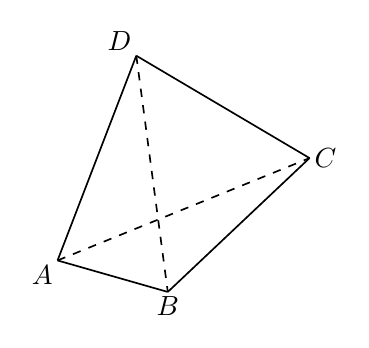
\begin{tikzpicture}[scale=1.0, semithick, every node/.style={inner sep=1.5pt}]
  \coordinate (D) at (2.0,3.2);
  \coordinate (A) at (1.0,0.6);
  \coordinate (C) at (4.2,1.9);
  \coordinate (B) at (2.4,0.2);
  \draw (D) -- (A);
  \draw (D) -- (C);
  \draw (C) -- (B);
  \draw (A) -- (B);
  \draw[dashed] (A) -- (C);
  \draw[dashed] (D) -- (B);
  \node[above left] at (D) {$D$};
  \node[below left] at (A) {$A$};
  \node[right] at (C) {$C$};
  \node[below] at (B) {$B$};
\end{tikzpicture}
\end{center}
\nopagebreak[4]
\end{question}
\gkpart{二、选择题}

\begin{question}
\gkti{15}若 $1+\sqrt2\mathrm i$ 是关于 $x$ 的实系数方程 $x^2+bx+c=0$ 的一个复数根，则\mbox{（　　）}

（A）$b=2$，$c=3$

（B）$b=-2$，$c=3$

（C）$b=-2$，$c=-1$

（D）$b=2$，$c=-1$

\end{question}
\begin{question}
\gkti{16}在 $\triangle ABC$ 中，若 $\sin^2A+\sin^2B<\sin^2C$，则 $\triangle ABC$ 的形状是\mbox{（　　）}

（A）锐角三角形

（B）直角三角形

（C）钝角三角形

（D）不能确定

\end{question}
\begin{question}
\gkti{17}设 $10\leqslant x_1<x_2<x_3<x_4\leqslant10^4$，$x_5=10^5$。随机变量 $\xi_1$ 取值 $x_1$，$x_2$，$x_3$，$x_4$，$x_5$ 的概率均为 $0.2$，随机变量 $\xi_2$ 取值 $\dfrac{x_1+x_2}2$，$\dfrac{x_2+x_3}2$，$\dfrac{x_3+x_4}2$，$\dfrac{x_4+x_5}2$，$\dfrac{x_5+x_1}2$ 的概率也均为 $0.2$。若记 $D\xi_1$，$D\xi_2$ 分别为 $\xi_1$，$\xi_2$ 的方差，则\mbox{（　　）}

（A）$D\xi_1>D\xi_2$

（B）$D\xi_1=D\xi_2$

（C）$D\xi_1<D\xi_2$

（D）$D\xi_1$ 与 $D\xi_2$ 的大小关系与 $x_1$，$x_2$，$x_3$，$x_4$ 的取值有关

\end{question}
\begin{question}
\gkti{18}设 $a_n=\dfrac1n\sin\dfrac{n\pi}{25}$，$S_n=a_1+a_2+\cdots+a_n$。在 $S_1$，$S_2$，$\cdots$，$S_{100}$ 中，正数的个数是\mbox{（　　）}

（A）$25$

（B）$50$

（C）$75$

（D）$100$

\end{question}
\gkpart{三、解答题}

\Needspace{0.4\textheight}
\begin{question}
\gkti{19}如图，在四棱锥 $P-ABCD$ 中，底面 $ABCD$ 是矩形，$PA\perp$ 底面 $ABCD$，$E$ 是 $PC$ 的中点。已知 $AB=2$，$AD=2\sqrt2$，$PA=2$。求：

（1） 三角形 $PCD$ 的面积；

（2） 异面直线 $BC$ 与 $AE$ 所成角的大小。
\nopagebreak[4]
\begin{center}% 2012 年上海卷理科第 19 题：四棱锥 P-ABCD，PA⊥底面 ABCD，E 为 PC 中点。
% 来源 PDF：普通高考/2012/2012上海理.pdf，第 1 页（印面 767）第 3 栏。
% 重绘依据：原图为斜二测式透视：A、B 在前，C、D 在后，P 在 A 的正上方；E 在 PC 上；
%   实线 PA、PB、PC、PD、AB、BC，虚线 AD、CD、AC 与 AE。
\begin{tikzpicture}[scale=0.95, semithick, every node/.style={inner sep=1.5pt}]
  \coordinate (A) at (0.2,0.4);
  \coordinate (B) at (3.0,0.0);
  \coordinate (C) at (4.0,1.5);
  \coordinate (D) at (1.2,1.9);
  \coordinate (P) at (0.2,3.8);
  \coordinate (E) at ($(P)!0.5!(C)$);
  \draw (P) -- (A);
  \draw (P) -- (B);
  \draw (P) -- (C);
  \draw (P) -- (D);
  \draw (A) -- (B) -- (C);
  \draw[dashed] (A) -- (D) -- (C);
  \draw[dashed] (A) -- (C);
  \draw[dashed] (A) -- (E);
  \node[left] at (A) {$A$};
  \node[below] at (B) {$B$};
  \node[right] at (C) {$C$};
  \node[above left] at (D) {$D$};
  \node[above] at (P) {$P$};
  \node[right] at ([xshift=2pt]E) {$E$};
\end{tikzpicture}
\end{center}
\nopagebreak[4]
\end{question}
\begin{question}
\gkti{20}已知函数 $f(x)=\lg(x+1)$。

（1） 若 $0<f(1-2x)-f(x)<1$，求 $x$ 的取值范围；

（2） 若 $g(x)$ 是以 $2$ 为周期的偶函数，且当 $0\leqslant x\leqslant1$ 时，有 $g(x)=f(x)$，求函数 $y=g(x)$（$x\in[1,2]$）的反函数。

\Needspace{0.4\textheight}
\end{question}
\begin{question}
\gkti{21}海事救援船对一艘失事船进行定位：以失事船的当前位置为原点，以正北方向为 $y$ 轴正方向建立平面直角坐标系（以 $1$ 海里为单位长度），则救援船恰好在失事船正南方向 $12$ 海里 $A$ 处，如图。现假设：①失事船的移动路径可视为抛物线 $y=\dfrac{12}{49}x^2$；②定位后救援船即刻沿直线匀速前往救援；③救援船出发 $t$ 小时后，失事船所在位置的横坐标为 $7t$。

（1） 当 $t=0.5$ 时，写出失事船所在位置 $P$ 的纵坐标。若此时两船恰好会合，求救援船速度的大小和方向；

（2） 问救援船的时速至少是多少海里才能追上失事船？
\nopagebreak[4]
\begin{center}% 2012 年上海卷理科第 21 题：失事船路径 y=12x^2/49，救援船出发点 A(0,-12)。
% 来源 PDF：普通高考/2012/2012上海理.pdf，第 2 页（印面 768）第 1 栏。
% 重绘依据：原图为平面直角坐标系：y 轴向上过 O、A，A 在负 y 轴；抛物线开口向上过 O，
%   右支上标点 P，A 与 P 连直线，x 轴正向朝右。
\begin{tikzpicture}[scale=0.33, semithick, >=Stealth]
  \draw[->] (-4.6,0) -- (5.0,0) node[below] {$x$};
  \draw[->] (0,-14.6) -- (0,6.0) node[left] {$y$};
  \node[below left] at (0,0) {$O$};
  \draw[domain=-4.6:4.6, samples=120] plot (\x, {12*\x*\x/49});
  \coordinate (A) at (0,-12);
  \coordinate (P) at (3.5,3);
  \fill (A) circle (2pt) node[left] {$A$};
  \fill (P) circle (2pt) node[right] {$P$};
  \draw (A) -- (P);
\end{tikzpicture}
\end{center}
\nopagebreak[4]
\end{question}
\begin{question}
\gkti{22}在平面直角坐标系 $xOy$ 中，已知双曲线 $C_1:2x^2-y^2=1$。

（1） 过 $C_1$ 的左顶点引 $C_1$ 的一条渐近线的平行线，求该直线与另一条渐近线及 $x$ 轴围成的三角形的面积；

（2） 设斜率为 $1$ 的直线 $l$ 交 $C_1$ 于 $P$，$Q$ 两点。若 $l$ 与圆 $x^2+y^2=1$ 相切，求证：$OP\perp OQ$；

（3） 设椭圆 $C_2:4x^2+y^2=1$。若 $M$，$N$ 分别是 $C_1$，$C_2$ 上的动点，且 $OM\perp ON$，求证：$O$ 到直线 $MN$ 的距离是定值。

\end{question}
\begin{question}
\gkti{23}对于数集 $X=\{-1,x_1,x_2,\cdots,x_n\}$，其中 $0<x_1<x_2<\cdots<x_n$，$n\geqslant2$，定义向量集 $Y=\{\overrightarrow a\mid\overrightarrow a=(s,t),\ s\in X,\ t\in X\}$。若对任意 $\overrightarrow{a_1}\in Y$，存在 $\overrightarrow{a_2}\in Y$，使得 $\overrightarrow{a_1}\cdot\overrightarrow{a_2}=0$，则称 $X$ 具有性质 $P$。例如 $\{-1,1,2\}$ 具有性质 $P$。

（1） 若 $x>2$，且 $\{-1,1,2,x\}$ 具有性质 $P$，求 $x$ 的值；

（2） 若 $X$ 具有性质 $P$，求证：$1\in X$，且当 $x_n>1$ 时，$x_1=1$；

（3） 若 $X$ 具有性质 $P$，且 $x_1=1$，$x_2=q$（$q$ 为常数），求有穷数列 $x_1$，$x_2$，$\cdots$，$x_n$ 的通项公式。

\Needspace{9\baselineskip}

\end{question}